\documentclass{IEEEtran}
\usepackage[spanish]{babel} % Definir el idioma del documento
\usepackage[letterpaper,top = 2cm, bottom = 2cm, left = 2cm, right = 2cm, marginparwidth = 1.75cm]{geometry} % Especificar los márgenes según la norma
\usepackage{pdfpages} % Añadir PDFs y que te cuente las páginas para el documento
\usepackage{subfiles} % Tener subdocumentos (hay más opciones)
\usepackage{tableof} % Se utiliza para los indices de los subdocumentos
\usepackage{float} % Para usar lo de 'H'
\usepackage{fancyhdr}
\usepackage{comment}
\usepackage{biblatex} % Paquete para manejar citas y bibliografía
\usepackage{amsmath}
\addbibresource{bibliografia.bib} % Cargar el archivo .bib

\def\TituloProyecto{Puente de Cody Docks}
\def\Autor{Mercedes Román Ruiz}
\def\Asignatura{Ampliación de Mecánica}
\def\Curso{2024 - 25}
\def\Fecha{Mayo 2024}

\begin{document}
\sloppy 
\setlength{\parindent}{30pt}
\setlength{\parskip}{6pt}
\renewcommand\thesection{\arabic{section}}
\renewcommand{\baselinestretch}{1.5}

\begin{titlepage}
    \centering
    
\includegraphics[width=0.5\linewidth]{Imagenes/Logo UPM.png} \par
    \vspace{1cm}
    {\bfseries\LARGE Escuela Técnica Superior de Ingenieros Industriales \par}
    \vspace{0.5cm}
    {\scshape\Large Máster en Ingeniería Industrial \par}
    \vspace{3 cm}
    {\Huge \textbf{\TituloProyecto} \par}
    \vfill
    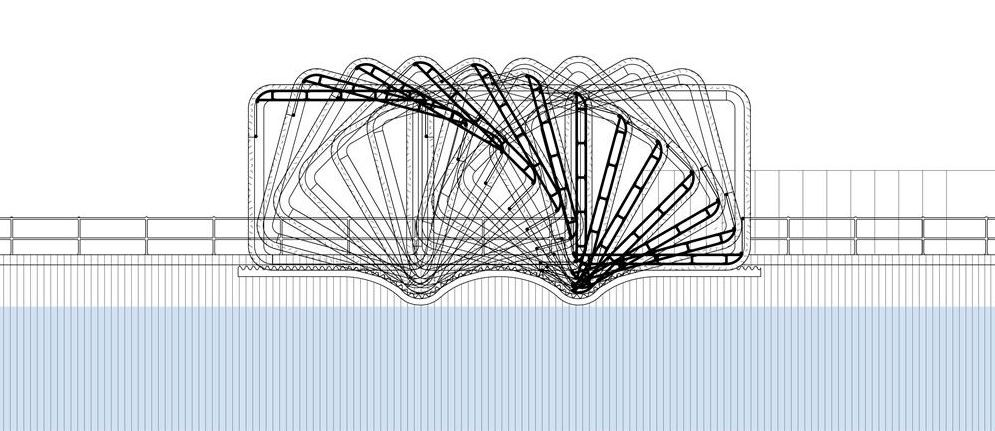
\includegraphics[width=0.5\linewidth]{Imagenes/Puente de Cody Docks.jpg} \par
    \vfill
    {\Large Autora: Mercedes Román Ruiz \par}
    {\Large \Asignatura \  \Curso \par}
    {\Large \Fecha \par}
\end{titlepage}

\tableofcontents

\section{El Innovador Puente Rodante de Cody Dock: Una Solución Urbana Sostenible}

El Puente Rodante de Cody Dock (Figura \ref{fig: Dibujo de Cody Dock}), diseñado por Thomas Randall-Page, representa una solución de ingeniería notable para superar las limitaciones espaciales y presupuestarias comunes en entornos urbanos densos como Londres. Su principal innovación radica en un sistema de rodadura completa que permite la rotación del puente sobre sí mismo para facilitar el paso de embarcaciones, eliminando la necesidad de los complejos y costosos sistemas eléctricos o hidráulicos presentes en los puentes móviles convencionales. Esta característica distintiva subraya su eficiencia y adaptabilidad en contextos urbanos consolidados.

\begin{figure}[h]
    \centering
    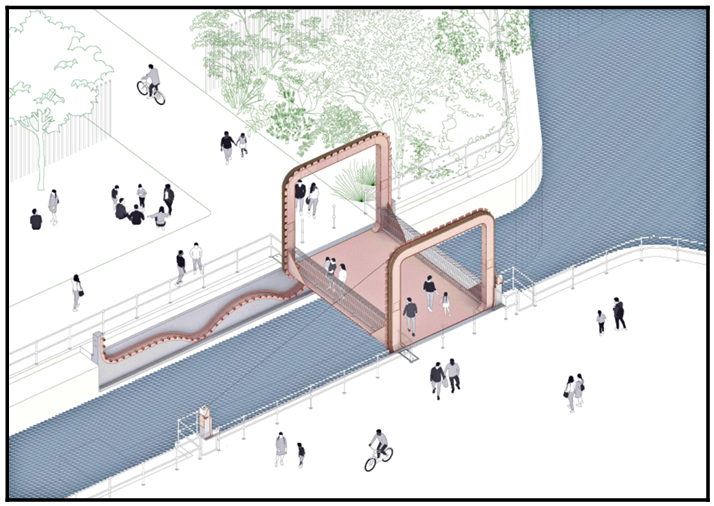
\includegraphics[width = 0.5 \textwidth]{Imagenes/Cody Dock Sketch.png}
    \caption{Boceto del Puente - Thomas Randall-Page \cite{randallpage2021}.}
    \label{fig: Dibujo de Cody Dock}
\end{figure}

\section{Fundamentos Teóricos: Del Descubrimiento de Maxwell a la Aplicación de Robison}

La singularidad del diseño del Puente de Cody Dock no es casualidad, sino que se basa en principios matemáticos bien establecidos. En 1849, James Clerk Maxwell realizó un descubrimiento fundamental al demostrar que una línea recta puede rodar suavemente sobre una catenaria invertida. Posteriormente, en 1960, G. Robison extendió esta idea al probar que un cuadrado también puede rodar suavemente sobre una secuencia de catenarias truncadas y unidas. Para hacer tangible esta teoría, Stan Wagon construyó en 1997 un triciclo funcional con ruedas cuadradas, un logro que capturó la atención mediática (Fig. \ref{fig: Ripley's Belive It or Not}). Estos hallazgos teóricos sentaron las bases para que Randall-Page concibiera el Puente de Cody Dock como una plataforma unida a dos grandes estructuras cuadradas, permitiendo una rotación fluida hasta alcanzar una posición invertida.

\begin{figure}[h]
    \centering
    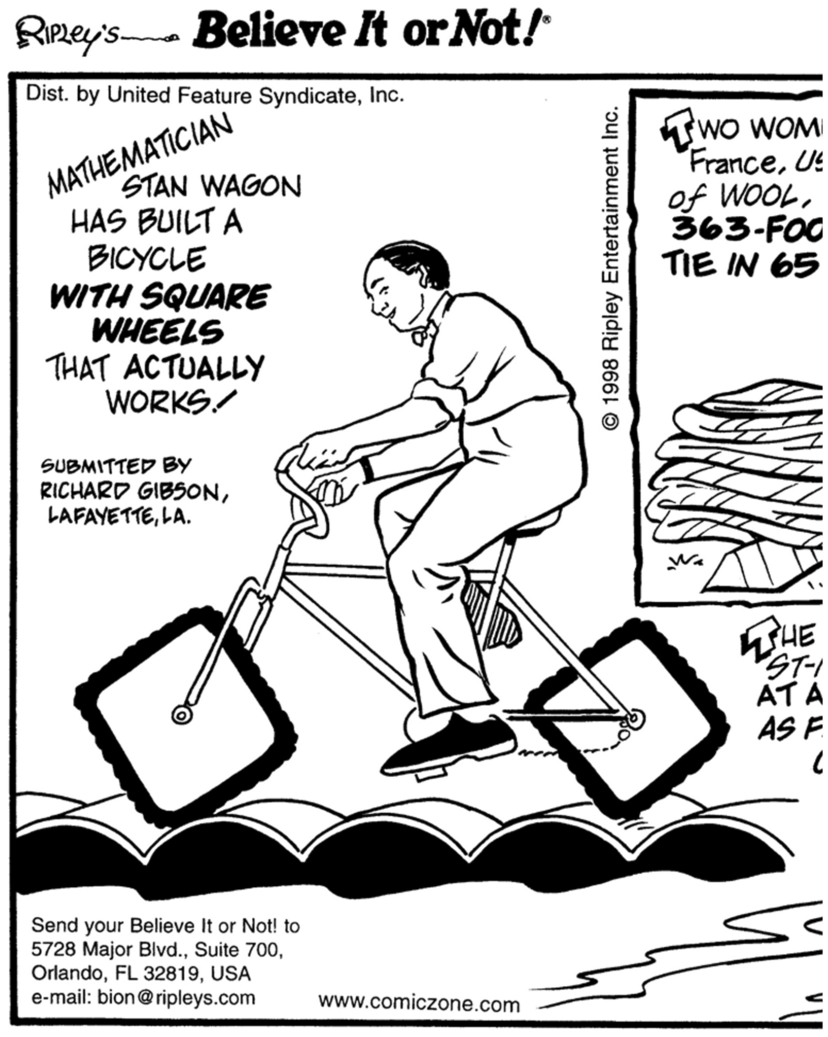
\includegraphics[width = 0.5 \textwidth]{Imagenes/Square Wheel Tricycle.png}
    \caption{Publicación sobre la bicicleta de rueda cuadrada en Ripley's Belive It or Not.}
    \label{fig: Ripley's Belive It or Not}
\end{figure}


\subsection{La Teoría del Rodamiento de Curvas de Maxwell}

En su influyente artículo \textit{``On the Theory of Rolling Curves''}, presentado a la Royal Society of Edinburgh, Maxwell exploró las propiedades geométricas de las curvas generadas por el rodamiento de una curva sobre otra. Este trabajo seminal proporcionó el marco teórico para aplicaciones futuras, incluyendo el diseño del puente de Cody Dock.

Mientras que el movimiento de una rueda circular perfecta ($r(\theta) = 1$) rodando sobre una superficie plana ($y = -1$) describe una trayectoria sencilla ($x(\theta) = \theta + \frac{\pi}{2}$), Maxwell se centró en un caso más complejo: una línea recta infinita ($x = -1$) con su centro de masa en el origen $(0,0)$. Su análisis reveló que dicha línea, definida en coordenadas polares como $r = a \sec \theta$, al rodar sobre una catenaria con parámetro $a$, traza una línea cuya distancia desde el vértice es también $a$.

Aplicando este principio a una línea horizontal ($r = -\csc \theta$ para $-\pi < \theta < 0$), la forma de la carretera sobre la que rueda se determina mediante la integración:

\[
x(\theta) = \int_{-\pi/2}^{\theta} -\csc t \, dt = \ln\left(-\cot\left(\frac{\theta}{2}\right)\right).
\]

La transformación de esta expresión paramétrica a su forma explícita ($y = f(x)$) se logra invirtiendo la relación para obtener $\theta = -2 \arctan(e^{-x})$ y sustituyéndola en la ecuación de la carretera ($y = -\csc \theta$), lo que revela la identidad fundamental de la catenaria invertida:

\[
y = -\cosh x.
\]

La Figura \ref{fig: A line rolling along a catenary} ilustra este elegante concepto. Sin embargo, el trabajo inicial de Maxwell no consideró la posibilidad de truncar la línea recta para crear ruedas poligonales, una extensión crucial que sería desarrollada posteriormente por Robison.

\begin{figure}[h]
    \centering
    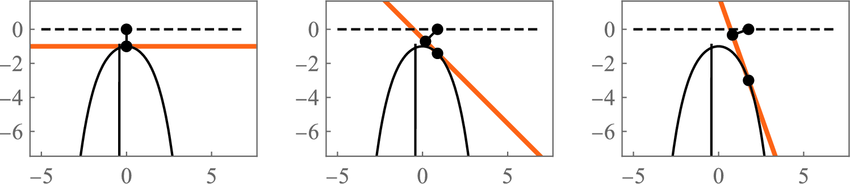
\includegraphics[width = 0.5 \textwidth]{Imagenes/A line rolling along a catenary.png}
    \caption{Línea que rueda a lo largo de una catenaria.}
    \label{fig: A line rolling along a catenary}
\end{figure}

\subsection{La Extensión de Robison: La Rueda Cuadrada y su Aplicación}

En 1960, Robison retomó el descubrimiento de Maxwell y lo extendió de manera ingeniosa para diseñar una rueda de forma cuadrada. Su idea clave consistió en truncar la catenaria en los puntos donde su pendiente es $\pm 1$. En estos puntos, la catenaria forma un ángulo de $45^\circ$ con la vertical, permitiendo que la unión de dos copias truncadas genere una cúspide de $90^\circ$, ideal para encajar con la esquina de un cuadrado (Figura \ref{fig: A square rolls smoothly along linked catenaries}).

Dado que la derivada de $\cosh x$ es $\sinh x$, las cúspides se producen en $x = \pm \operatorname{arsinh}(1) \approx \pm 0.88$. Esta configuración permite que el cuadrado ruede sobre esta carretera manteniendo su centro de masa a una altura constante, lo que implica un movimiento dinámicamente equivalente al de un círculo rodando sobre una superficie plana, sin trabajo neto contra la gravedad.

Este modelo teórico no solo permite diseñar la forma de la carretera, sino también la rueda cuadrada que se desplaza con una sorprendente suavidad. Aunque la relación entre la posición horizontal ($x$) y el parámetro angular ($\theta$) no es estrictamente lineal, la desviación de la linealidad es lo suficientemente pequeña como para que no sea perceptible en la práctica si se aplica una velocidad angular constante al cuadrado.

\begin{figure}[h]
    \centering
    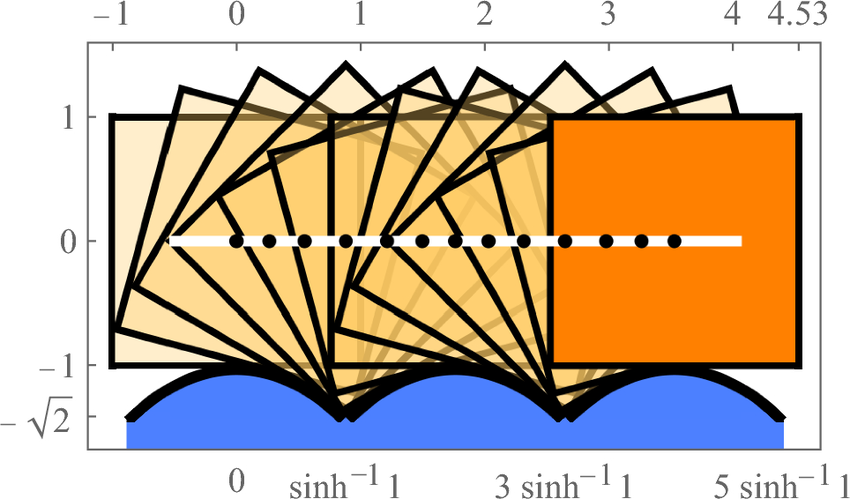
\includegraphics[width = 0.5 \textwidth]{Imagenes/A square rolls smoothly along linked catenaries.png}
    \caption{Cuadrado rodando suavemente a lo largo de catenarias conectadas.}
    \label{fig: A square rolls smoothly along linked catenaries}
\end{figure}

\section{Diseño y Funcionamiento del Puente de Cody Dock}

El diseño del Puente de Cody Dock se inspira directamente en estos principios teóricos. Para guiar la estructura rodante de acero de manera precisa, se utilizan dientes y pasadores. La necesidad de un encaje perfecto implica la eliminación de los ángulos rectos, lo cual se logra mediante el redondeo de las esquinas utilizando cuartos de círculo, una solución geométrica natural.

\subsection{Geometría y Mecanismo de Rodadura}

La estructura principal del puente consiste en una sección tubular circular de acero, construida con perfiles huecos soldados. El radio de curvatura del puente coincide exactamente con el de los rieles de soporte, asegurando una rotación suave alrededor de un eje horizontal. La geometría fue cuidadosamente optimizada para mantener el centro de masas de la estructura dentro del radio de rodadura, lo que facilita su operación manual.

El puente gira sobre dos rieles semicirculares mediante un sistema de engranajes y manivelas, prescindiendo de sistemas electrónicos o motores. Para minimizar el esfuerzo necesario para la rotación, se incorporaron contrapesos y se logró un equilibrado estructural preciso.

\subsection{Las Matemáticas de las Esquinas Redondeadas}

Para las esquinas redondeadas del puente, se considera una rueda circular de radio $1$, con su centro de masa en el origen $(0, 0)$ y su centro geométrico en $(0, y_0)$, donde $y_0 \leq -1$. La parametrización de la carretera sobre la que rueda esta sección se describe mediante las siguientes ecuaciones:

\[ x(t) = \int_{0}^{t}{\frac{g_1(s) g_2'(s) - g_1'(s) g_2(s)}{\sqrt{g_1(s)^2 + g_2(s)^2}}} \, ds \]
\[ y(t) = - \sqrt{g_1(t)^2 + g_2(t)^2} \]

Donde la rueda circular se parametriza como $g(t) = (\sin t, y_0 - \cos t)$, lo que lleva a:

\[ x(t) = \int_{0}^{t}\frac{1 - y_0 \cos s}{\sqrt{1 + y_0^2 - 2 y_0 \cos s}} \, ds \]
\[ y(t) = - \sqrt{1 + y_0^2 - 2 y_0 \cos t} \]

La evaluación de la integral de $x(t)$ involucra un cambio de variable y el uso de integrales elípticas de Legendre ($E$ y $F$), resultando en:

\begin{equation*}
    \resizebox{0.5 \textwidth}{!}{$x(t) = (1 - y_0) E \left( \frac{t}{2} \Big| - \frac{4y_0}{(1 - y_0)^2} \right) + (1 + y_0) F \left( \frac{t}{2} \Big| - \frac{4 y_0}{(1 - y_0)^2} \right)$}
\end{equation*}

\[ y(t) = - \sqrt{1 + y_0^2 - 2 y_0 \cos t} \]

La carretera resultante es una secuencia de bucles. Aunque la construcción física completa de esta curva es inviable, el diseño del puente solo requiere una porción específica para las esquinas redondeadas. La carretera final del puente es una combinación de segmentos de catenarias ($y = - \cosh x$) para las secciones rectas y segmentos derivados de estos bucles para las esquinas redondeadas. Un enfoque simplificado, basado principalmente en la integral elíptica $E$, fue crucial para el diseño práctico.

\section{Contexto Urbano, Histórico y Comunitario}

Cody Dock, ubicado en el East London a lo largo del río Lea, se encuentra en una antigua zona industrial en proceso de revitalización hacia un espacio comunitario y ecológico. La necesidad de una conexión peatonal permanente que a su vez permitiera el paso ocasional de embarcaciones por el canal impulsó este proyecto. Enmarcado en un proceso de regeneración urbana con una fuerte participación ciudadana y financiación colectiva, el diseño del puente debía cumplir con criterios de bajo impacto ambiental, mantenimiento mínimo y alta fiabilidad. La activa inclusión de la comunidad local en las fases de diseño y construcción, con voluntarios colaborando incluso en la operación diaria, fortaleció el sentido de pertenencia y el cuidado de esta infraestructura urbana.

\section{Análisis Mecánico, Estructural y de Sostenibilidad}

Desde una perspectiva mecánica y estructural, el puente puede analizarse como un cilindro hueco sometido a cargas distribuidas por su peso propio y la carga peatonal. Los modelos de elementos finitos confirmaron su capacidad para resistir las cargas máximas tanto en posición horizontal como durante la rotación. Se identificaron puntos críticos de concentración de tensiones en las áreas de apoyo sobre los rieles y en las uniones estructurales, los cuales fueron reforzados con conectores soldados y cartelas triangulares para optimizar la distribución de las cargas.

La sostenibilidad fue un principio rector en el diseño y la construcción. La operación manual del puente elimina el consumo energético asociado a sistemas motorizados. Se priorizó el uso de acero estructural S275, conocido por su resistencia, soldabilidad y durabilidad, así como madera reciclada tratada para el tablero. El proceso de montaje modular, con prefabricación en taller y ensamblaje in situ, minimizó la necesidad de maquinaria pesada y redujo el impacto ambiental. Además, el diseño busca un mantenimiento mínimo, realizable por personal no especializado.

\section{Limitaciones, Consideraciones Técnicas y Potencial de Replicabilidad}

A pesar de sus numerosas ventajas, el sistema presenta ciertas limitaciones. No es adecuado para tráfico rodado pesado y requiere inspecciones periódicas para prevenir la corrosión del acero. La operación manual podría no ser viable para personas con discapacidad o en condiciones climáticas extremas. Por ello, su uso se recomienda principalmente para zonas peatonales, vías verdes y entornos urbanos con bajo tráfico.

No obstante, el diseño del Puente Rodante de Cody Dock posee un significativo potencial de replicabilidad. Su escala, los materiales empleados y el modo de operación pueden adaptarse a diferentes localizaciones. Su bajo coste y la relativa simplicidad de su construcción lo convierten en una opción viable para proyectos de regeneración urbana o iniciativas de movilidad sostenible en diversos contextos.

\section{Conclusión}

El Puente Rodante de Cody Dock representa una innovadora convergencia de principios de la mecánica clásica y objetivos de sostenibilidad y participación comunitaria en el diseño de infraestructuras urbanas móviles. Su concepción y ejecución lo erigen como un ejemplo inspirador para futuras intervenciones de ingeniería que buscan soluciones eficientes, de bajo impacto y con un fuerte sentido de pertenencia para la comunidad.

\nocite{*}
\printbibliography

\end{document}